% Gemini theme
% https://github.com/anishathalye/gemini
%
% We try to keep this Overleaf template in sync with the canonical source on
% GitHub, but it's recommended that you obtain the template directly from
% GitHub to ensure that you are using the latest version.

\documentclass[final, 20pt]{beamer}

% ====================
% Packages
% ====================

\usepackage[T1]{fontenc}
\usepackage{lmodern}
% Poster dimensions
\usepackage[size=custom,width=120,height=85,scale=1.0]{beamerposter}
% Set font size
\setbeamerfont{block body}{family=\Lato,size={\fontsize{30}{40}}}
\usepackage[font=normalsize]{caption}

\usetheme{gemini}
\usecolortheme{gemini}
\usepackage{csquotes}
\usepackage[font=large]{subfig}
\usepackage{graphicx}
\usepackage{booktabs}
\usepackage{tikz}
\usepackage{pgfplots}
\pgfplotsset{compat=1.14}

% For math
\usepackage{amsmath}
\usepackage{amsthm}
\usepackage{amssymb}
\usepackage{bbm}


% ====================
% Lengths
% ====================

% If you have N columns, choose \sepwidth and \colwidth such that
% (N+1)*\sepwidth + N*\colwidth = \paperwidth
\newlength{\sepwidth}
\newlength{\colwidth}
\setlength{\sepwidth}{0.025\paperwidth}
\setlength{\colwidth}{0.45\paperwidth}

\newcommand{\separatorcolumn}{\begin{column}{\sepwidth}\end{column}}

% ====================
% Title
% ====================

\title{Implicit Regularization in Deep Learning: The Kernel and Rich Regimes}

\author{Henry Smith\\Advised by Professor Harrison Zhou}

\institute[shortinst]{Yale University}

\footercontent{
\hfill Department of Statistics \& Data Science \hfill 
henry.smith@yale.edu \hfill}
% ====================
% Body
% ====================

\begin{document}

\begin{frame}[t]
\begin{columns}[t]
\separatorcolumn

\begin{column}{\colwidth}
 
  \begin{block}{Motivation}
  Over the past couple of decades, neural networks have risen through the ranks to replace random forests and SVMs as the premier models for prediction. In large part, this proliferation in deep learning models has been due to their good generalization properties. From a theoretical perspective, though, little is known as to why neural networks generalize so well. In our research, we examine two limits present in neural network training, the \enquote{kernel} and \enquote{rich} limits. Principally, we are interested in what these limits tell us about the generalization properties of neural networks.
  \end{block}

  \begin{block}{Introduction to the Kernel and Rich Limits}

    \heading{Problem Setup}
    Consider a differentiable model $h: \boldsymbol{w} \mapsto f(\boldsymbol{w}, \boldsymbol{x})$ which maps each weight vector $\boldsymbol{w} \in \mathbb{R}^p$ to a neural network function $f(\boldsymbol{w}, \cdot): \mathbb{R}^n \rightarrow \mathbb{R}$. Assume that the model $h$ is $D$-positive homogeneous, meaning $h(\alpha \boldsymbol{w}) = \alpha^D h(\boldsymbol{w})$ for each $\alpha > 0$. Also, suppose that we have some differentiable loss function $L$ which measures the misfit of each neural network function on our training data $\{ (\boldsymbol{x}_i, y_i) \}_{i=1}^N$.
    
    We would like to understand the \textbf{gradient flow} $(\boldsymbol{w}_{\alpha}(t))_{t \geq 0}$ on the objective $\frac{1}{\alpha^2}L(\alpha h(\boldsymbol{w}))$:
    \begin{align*}
    \boldsymbol{w}_{\alpha}'(t) = - \nabla\left( \frac{1}{\alpha^2}L(h(\boldsymbol{w}_{\alpha}(t))) \right) =  - \frac{1}{\alpha^2} Dh(\boldsymbol{w}_{\alpha}(t))^T \nabla L(h(\boldsymbol{w}_{\alpha}(t))), \quad \boldsymbol{w}_{\alpha}(0) = \alpha^{1/D}\boldsymbol{w}_0.
    \end{align*}
    From the practitioner's perspective, gradient flow is no more than a continuous time analog of gradient descent.
    
    \heading{Scaling Up}
    In particular, we are interested in what happens to the gradient flow solution $\boldsymbol{w}_{\alpha}^{\star} = \lim_{t \to \infty} \boldsymbol{w}_{\alpha}(t)$ when the scale $\alpha$ of the initialization $\boldsymbol{w}_{\alpha}(0) = \alpha^{1/D}\boldsymbol{w}_0$ grows arbitrarily large. Equivalently, what happens to the gradient flow when we initialize the weights our neural network to have larger and larger norm?
    
    The work of Chizat and colleagues demonstrates that in this limit $\alpha \rightarrow \infty$, training the model $h$ is equivalent to training the linearization of $h$ around its initialization $\boldsymbol{w}_{\alpha}(0)$ \cite{chizat2018lazy}. That is, training $h$, which may be highly nonconvex as a function of its weights $\boldsymbol{w} \in \mathbb{R}^p$, is simplified to training an affine model. This $\alpha \rightarrow \infty$ limit of network training is called the \textbf{kernel limit}.
    
    Conversely, when the scale of the initialization grows very small $\alpha \rightarrow 0$, training the model $h$ is very different from training the linearization of $h$ around its initialization. This is called the \textbf{rich limit} of network training.

    \begin{figure}
        \centering
        \subfloat[$\alpha = 10^{-1}$]{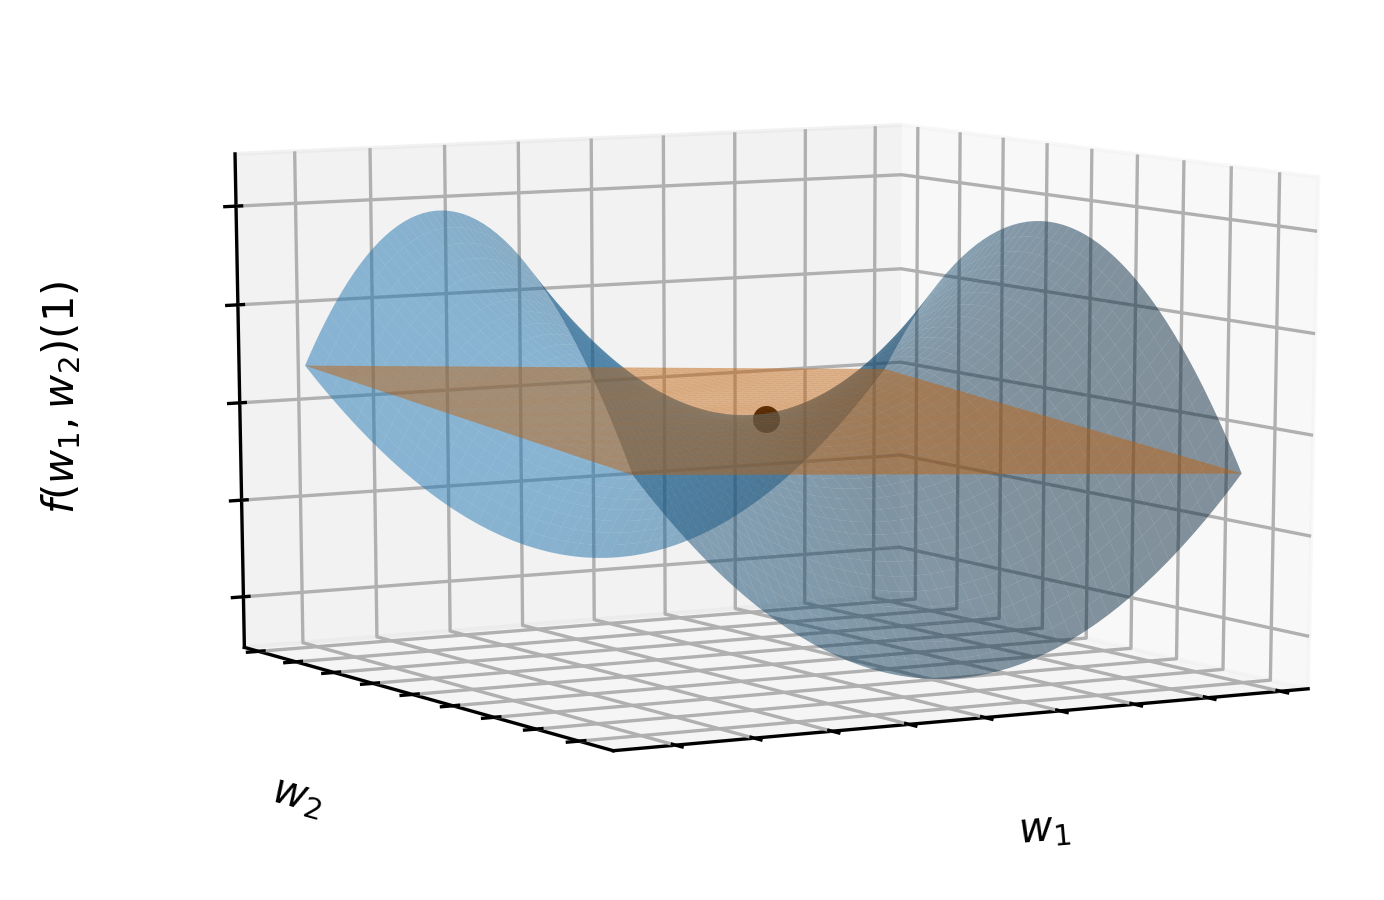
\includegraphics[width=.5\linewidth]{Poster/Poster_Imgs/visualize_linearized_0.1.png}}\hfill
        \subfloat[$\alpha = 10$]{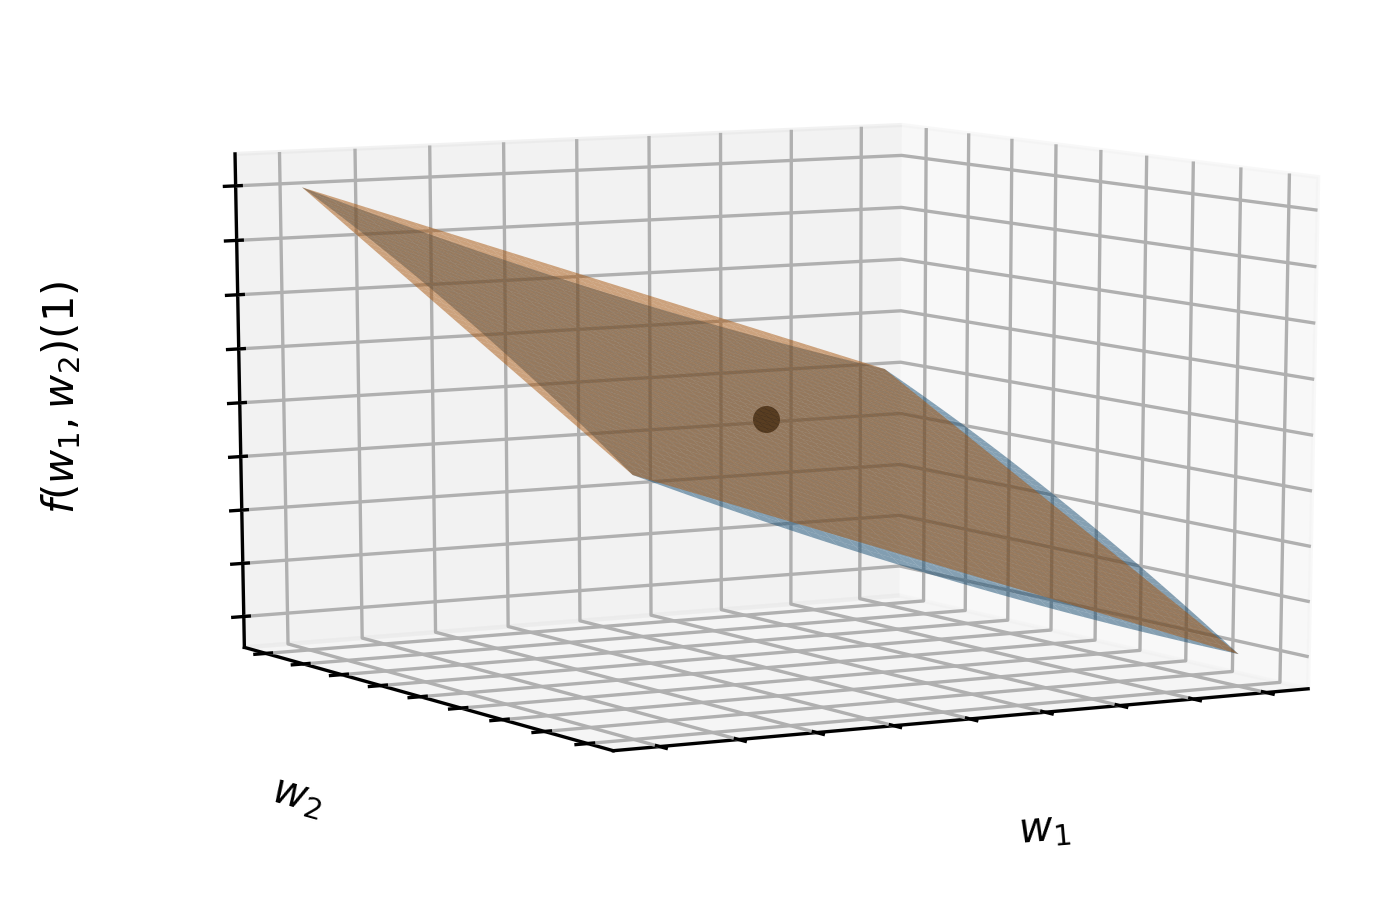
\includegraphics[width=.5\linewidth]{Poster/Poster_Imgs/visualize_linearized_10.png}}\hfill
        \caption{We plot a linear model $f(w_1, w_2, x) = (w_1^2 - w_2^2)x$ (blue) as a function of its weights $(w_1, w_2) \in \mathbb{R}^2$ at the fixed input $x = 1$. In addition, we visualize the linearization of the model $f(w_1, w_2, 1)$ around its initialization  $\boldsymbol{w}_{\alpha}(0) = \alpha \mathbbm{1}$, $\bar{f}(w_1, w_2, 1) = f(\boldsymbol{w}_{\alpha}(0)) + D_{(w_1, w_2)} f(\boldsymbol{w}_{\alpha}(0), \boldsymbol{x})\\ 
        \cdot ((w_1, w_2) - \boldsymbol{w}_{\alpha}(0))$ (orange). Notice that for (a),  $f(w_1, w_2, 1)$ is very different from $\bar{f}$ about $\boldsymbol{w}_{\alpha}(0)$, whereas for (b),  $f(w_1, w_2, 1)$ is very close to $\bar{f}$.}
        \label{fig:my_label}
    \end{figure}
  \end{block}
\end{column}
\separatorcolumn

\begin{column}{\colwidth}

    \begin{block}{Connection with Implicit Regularization}
    
    In \cite{woodworth2020kernel}, Woodworth and colleagues consider the linear regression model $f(\boldsymbol{w}, \boldsymbol{x}) = \langle \boldsymbol{\beta}_{\boldsymbol{w}}, \boldsymbol{x} \rangle$ with coefficient vector $\boldsymbol{\beta}_{\boldsymbol{w}} = \boldsymbol{w}_+^2 - \boldsymbol{w}_-^2$. Here, the weights of our neural network are $\boldsymbol{w} = [\boldsymbol{w}_+, \boldsymbol{w}_-]^T \in \mathbb{R}^{2n}$, and $\boldsymbol{v}^2$ denotes element-wise squaring of $\boldsymbol{v} \in \mathbb{R}^n$. They suppose that the loss function is the empirical risk $L(f(\boldsymbol{w}, \cdot)) = \sum_{i=1}^N [y_i - f(\boldsymbol{w}, \boldsymbol{x}_i)]^2$,
    where the training data $\{(\boldsymbol{x}_i, y_i) \}_{i=1}^N$ satisfies $N \ll n$. More precisely, they assume that there are many solutions to the system $\boldsymbol{X} \boldsymbol{\beta} = \boldsymbol{y}$. 
    
    For this particular linear regression problem, the gradient flow solution in the kernel limit $\alpha \rightarrow \infty$ corresponds to the minimum $\ell^2$ solution of the system $\boldsymbol{X} \boldsymbol{\beta} = \boldsymbol{y}$, whereas the solution in the rich limit $\alpha \rightarrow 0$ corresponds to the minimum $\ell^1$ solution \cite{woodworth2020kernel}. This result suggests the immense benefit of training near the rich limit for problems in which the input data $\boldsymbol{x} \in \mathbb{R}^n$ is very high-dimensional but is suspected to have implicit sparsity. 
    
    \end{block}
    
    \begin{block}{A New Example: The Logistic Regression Problem}
    
    \begin{figure}
        \centering
        \subfloat{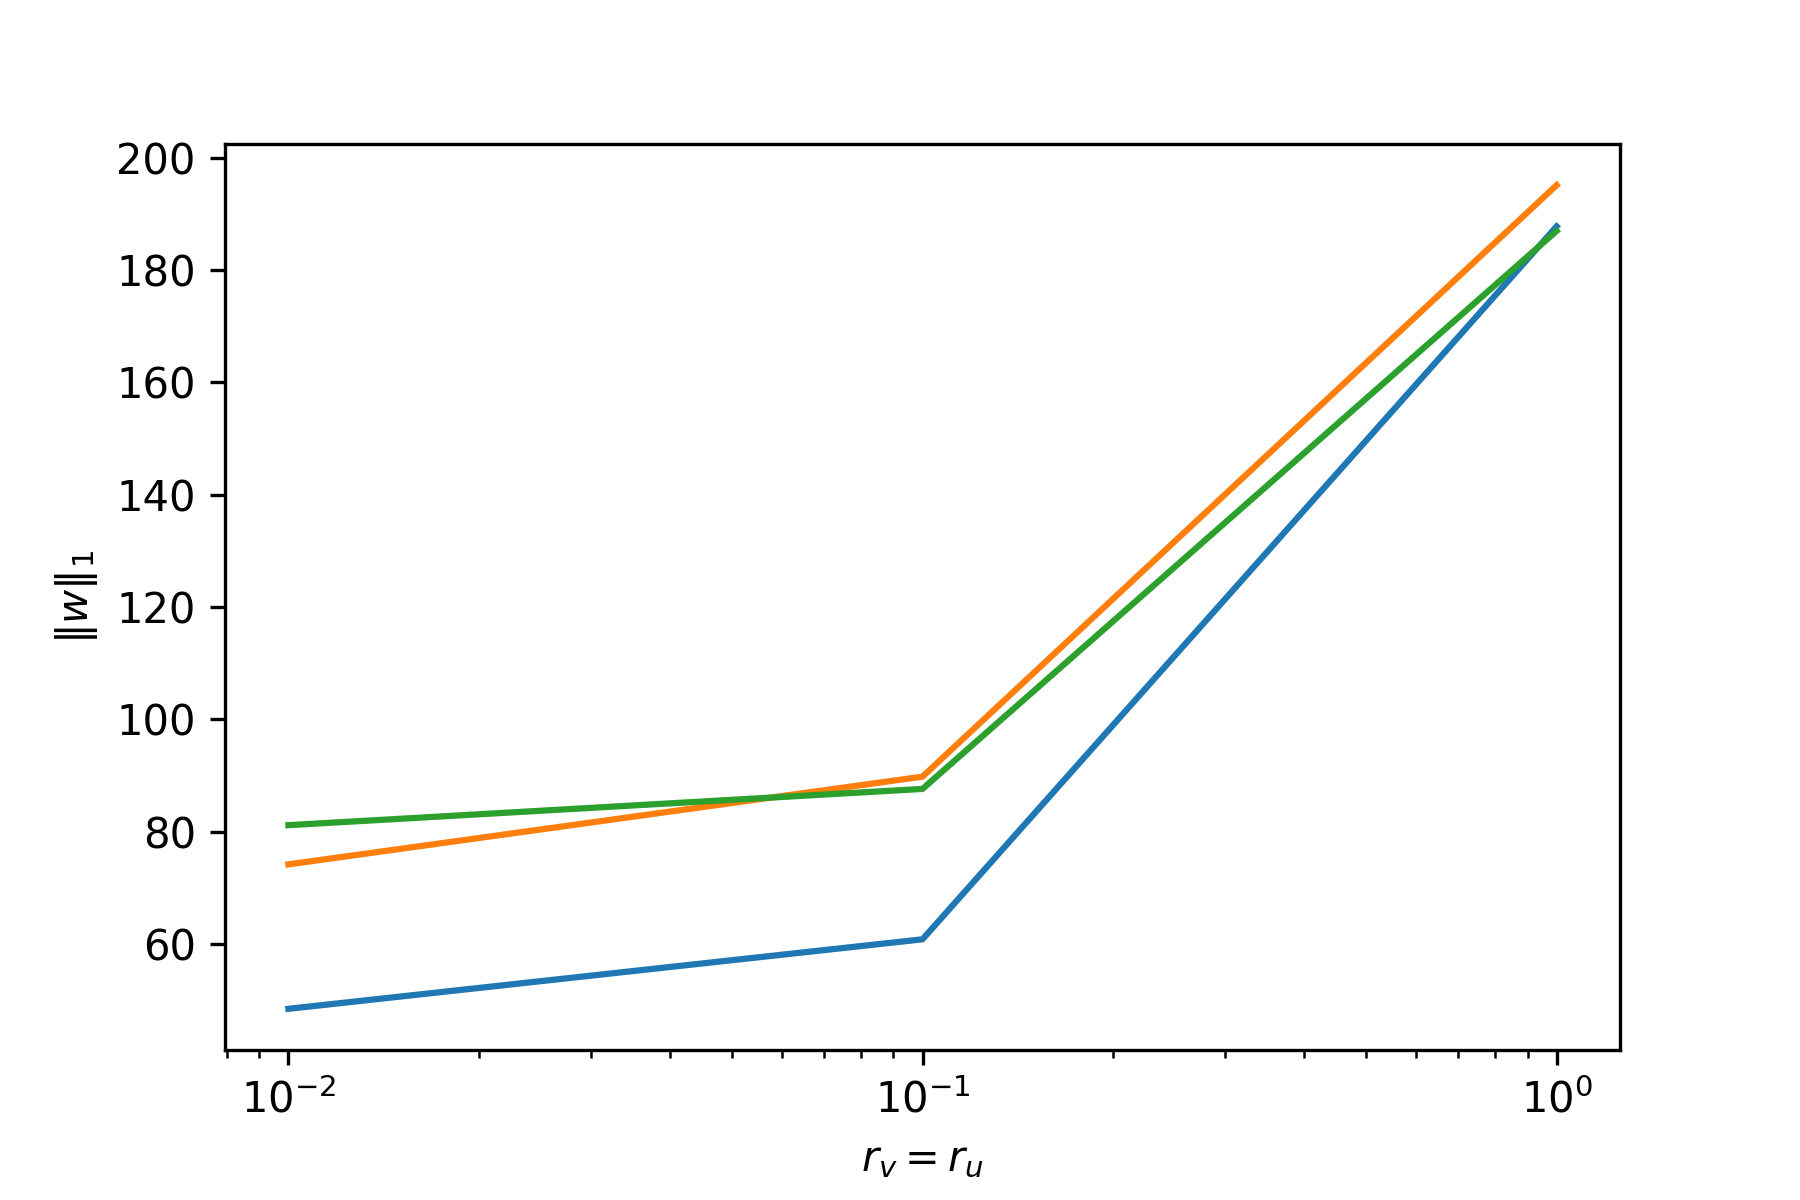
\includegraphics[width=.5\linewidth]{Imgs/Sparse Logistic Regression/param_l1_avg.png}}\hfill
        \subfloat{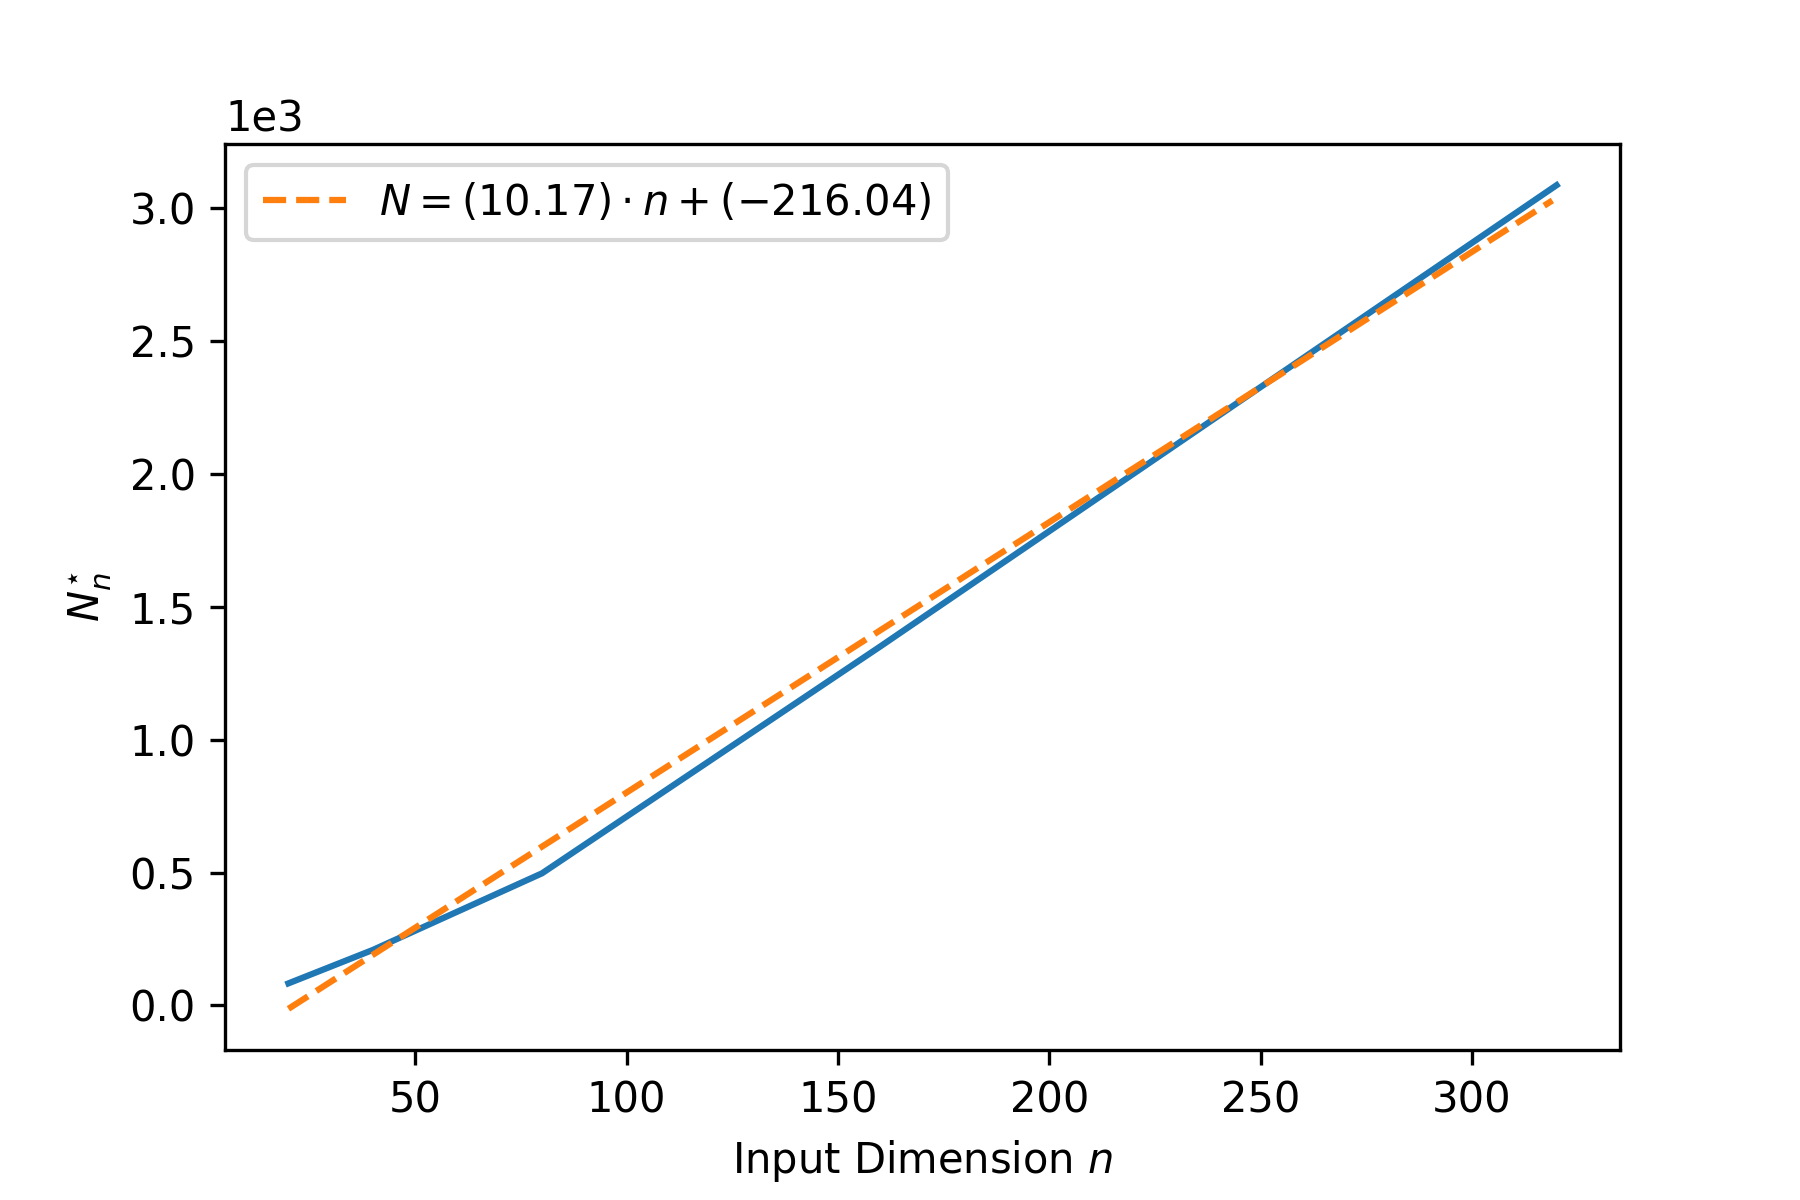
\includegraphics[width=.5\linewidth]{Imgs/Sparse Logistic Regression/min_N_60.png}}\hfill
        \caption{(left) The $\ell^1$ norm of the gradient descent solution vector, where the gradient descent path is initialized with scale $r_v = r_{\boldsymbol{u}}$. Since the starting point of gradient descent is random, we average over $K=20$ trials. (right) The smallest number of training samples necessary to attain test error $< 0.4$ for input dimension $n$. For this experiment, the initialization scale is $r_v = r_{\boldsymbol{u}} = 10^{-1}$, and so training is performed close to the rich limit.}
        \label{fig:my_label}
    \end{figure}
    
    To investigate whether or not training near the rich limit results in implicit $\ell^1$ regularization for more advanced problems, we consider the sparse logistic regression problem posed by Wei and colleagues \cite{wei2019regularization}. Specifically, we suppose that the data  $(\boldsymbol{x}, y) \sim \rho$ is generated such that only the first two coordinates of $\boldsymbol{x} \in \{+1, 0, -1\}^n$ determine $y \in \{+1, -1\}$. For our model, we choose a ReLU neural network with a single hidden layer containing $m$ hidden units: $f(\boldsymbol{w}, \boldsymbol{x}) = \sum_{i=1}^m v_i \cdot \text{max}\{0, \boldsymbol{u}_i^T\boldsymbol{x}\}$.
    The weights $\{(v_i, \boldsymbol{u}_i)\}_{i=1}^m$ of the network are initialized according to $v_i \sim \mathcal{N}(0, r_v^2), \ \boldsymbol{u}_i \sim \mathcal{N}(\boldsymbol{0}, r_{\boldsymbol{u}}^2 \mathbbm{I})$.
    
    Our experiments suggest that the rich limit $r_v, r_{\boldsymbol{u}} \rightarrow 0$, does, in fact, impose implicit $\ell^1$ regularization on the gradient descent solution. Even more remarkable, our empirical results provide evidence that the generalization error of the ReLU network trained in the rich limit is bounded by $\mathbb{P}_{(\boldsymbol{x}, y) \sim \rho}(f(\boldsymbol{w}, \boldsymbol{x})y \leq 0) \lesssim \sqrt{\frac{d}{n}}$. This is the same [asymptotic] bound on the generalization error that Wei and colleagues achieved by including an explicit $\ell^2$ regularizer in the loss function.
    
    That is, by simply decreasing the scale with which we initialize the network weights, we have achieved commensurate performance to when we use an explicit $\ell^2$ regularizer. This result points to the immense role of implicit regularization in neural network generalization, and it suggests the necessity of further research into the kernel and rich limits.
    \end{block}
  \begin{block}{References}
    \footnotesize{\bibliographystyle{plain}\bibliography{Poster/poster}}
  \end{block}

\end{column}

\separatorcolumn
\end{columns}

\end{frame}

\end{document}